% !TeX document-id = {d8b4925c-2057-42a4-b894-2f1a3f1b6345}
%!TeX TXS-program:compile = txs:///xelatex/[--shell-escape]
\documentclass[aspectratio=169]{beamer}	% TPU recommends 16:9 ratio, 4:3 may require some work with inner theme .sty file

% Style options:
% light --- light theme (default)
% dark --- dark theme
% enlogo --- english TPU logo {default}
% rulogo --- russian TPU logo

\usetheme[light, rulogo]{tpu}		% dark theme used as an example of optional argument

\usepackage[russian]{babel}		%uncomment this to work in russian
\usepackage[utf8]{inputenc}
\usepackage[T2A]{fontenc}

\usepackage{fontspec}

\setromanfont{Brygada1918}[
Path=./fonts/BrygadaFontFiles/,
Extension = .ttf,
UprightFont=*-Regular,
BoldFont=*-Bold,
ItalicFont=*-Italic,
BoldItalicFont=*-BoldItalic
]

\setsansfont{ALSSirius}[
Path=./fonts/ALSSiriusFiles/,
Extension = .otf,
UprightFont=*-Regular,
BoldFont=*-Bold,
%ItalicFont=*-Italic,
%BoldItalicFont=*-BoldItalic
]

\setmonofont{Consolas}[
Path=./fonts/ConsolasFontFiles/,
%Scale=0.85,
Extension = .ttf,
UprightFont=*-Regular,
BoldFont=*-Bold,
ItalicFont=*-Italic,
BoldItalicFont=*-BoldItalic
]

\usepackage[cache=false]{minted}
\usepackage{xcolor} % to access the named colour LightGray
\definecolor{LightGray}{gray}{0.9}
\definecolor{onedarkBckGr}{RGB}{40, 44, 52}

\usemintedstyle[python]{default}
\setminted[python]{
	fontsize=\scriptsize,
	escapeinside=||,
	mathescape=true,
	numbersep=5pt,
	gobble=2,
	linenos=false,
	frame=single,
	framesep=1mm,
	python3=true,
	bgcolor=backcolour,
}

\usemintedstyle[pycon]{default}
\setminted[pycon]{
	fontsize=\scriptsize,
	escapeinside=||,
	mathescape=true,
	numbersep=5pt,
	gobble=2,
	linenos=false,
	frame=single,
	framesep=1mm,
	python3=true,
	bgcolor=backcolour,
	linenos=true,
}

\usepackage{booktabs}	% good looking tables
\usepackage{multicol}	% text in multiple columns, useful for side-by-side text and pictures
\usepackage{hyperref}
%\usepackage{minted}
\usepackage{xcolor}
\definecolor{maroon}{cmyk}{0, 0.87, 0.68, 0.32}
\definecolor{halfgray}{gray}{0.55}
\definecolor{ipython_frame}{RGB}{207, 207, 207}
\definecolor{ipython_bg}{RGB}{247, 247, 247}
\definecolor{ipython_red}{RGB}{186, 33, 33}
\definecolor{ipython_green}{RGB}{0, 128, 0}
\definecolor{ipython_cyan}{RGB}{64, 128, 128}
\definecolor{ipython_purple}{RGB}{170, 34, 255}
\definecolor{linkcolor}{HTML}{0000FF} % цвет гиперссылок
\definecolor{urlcolor}{HTML}{800080} % цвет ссылок
\definecolor{backcolour}{rgb}{0.95,0.95,0.92}

\usepackage{wrapfig}
\usepackage{ragged2e}
\usepackage[nooneline]{caption}
\DeclareCaptionTextFormat{center}{\centering{#1}}
\captionsetup[table]{justification=raggedleft, 
	labelformat=empty,	
	labelsep=endash,  
	textformat=center, 
	position=top, 
	skip=5pt
}

\usepackage{amsmath}
\usepackage{amsfonts}
\usepackage{amssymb}

\hyphenpenalty=10000	% i don’t think hyphenation in presentations is a good idea, feel free to change however you like

\title{\LARGE{Системный анализ процессов химической технологии}}
\subtitle{Лабораторная работа 2 \\ Операторы управления потоком команд \\ в Python}
\author[]{Вячеслав Алексеевич Чузлов, \\
	к.т.н., доцент ОХИ ИШПР}
\date{\today}

\begin{document}

% notice usage of \titleframe and several other unconventional functions
% the reason being is custom backgrounds on these slides

\titleframe		% title

\tocframe{}		% this custom frame accepts options for ToC



\section{Логический тип данных}
\sectionframe


\begin{frame}[fragile]{Логический тип данных}
\scriptsize
\begin{itemize}

\item Для логического типа данных \mintinline{python}|bool| можно объявлять логические переменные, инициализируя их логическими значениями или присваивая им результат вычисления логических выражений.

\item Логических констант в Python две: \mintinline{python}|True| (истина) и \mintinline{python}|False| (ложь).
\end{itemize}

\begin{minted}[]{pycon}
>>> x = True

>>> y = False

>>> z = 2 > -1

>>> print(x, y, z)
(True, False, True)
\end{minted}

\vfill
\end{frame}


\section{Операции сравнения}
\sectionframe


\begin{frame}[fragile]{Операции сравнения}
\scriptsize
Логические выражения являются аналогом математической формулы, результатом его вычисления будет одна из двух логических констант~-- \mintinline{python}|True| или \mintinline{python}|False|.

\begin{table}[h!]
%\caption{Операции сравнения}
\centering
\begin{tabular}{|p{.45\textwidth}|p{.45\textwidth}|}
	\hline
	\textbf{Операция} & \textbf{Описание} \\
	\hline
	\mintinline{ipython}|x < y| & Меньше \\
	\mintinline{ipython}|x <= y| & Меньше или равно \\
	\mintinline{ipython}|x > y| & Больше \\
	\mintinline{ipython}|x >= y| & Больше или равно \\
	\mintinline{ipython}|x == y| & Равно \\
	\mintinline{ipython}|x != y| & Не равно \\
	\hline
\end{tabular}	
\end{table}

{\color{tpugreen}\textbullet} Приоритет операций сравнения ниже, чем у арифметических операций:

\begin{minted}{pycon}
>>> print(2 + 3 * 5 > 7 / 2 + 3.5)
True
\end{minted}
\vfill
\end{frame}


%\begin{frame}[fragile]{Операции сравнения}
%\scriptsize
%Операции сравнения в Python  сравнивают относительные величины своих операндов и возвращают результат логического типа, значение которого обычно используется для выбора следующего действия в более крупном операторе или программе:
%
%\begin{minted}{python}
%|In [1]:| 1 < 2       # Меньше
%|Out[1]: True|
%
%|In [2]:| 2.0 >= 1    # Больше или равно: число целого типа 1 
%   |...:|             # преобразуется к 1.0
%|Out[2]: True|
%
%|In [3]:| 3.0 == 3.0  # Значения равны
%|Out[3]: True|
%
%|In [4]:| 3.0 != 3.0  # Значения не равны
%|Out[4]: False|
%\end{minted}
%\vfill
%\end{frame}


\section{Логические операции}
\sectionframe


\begin{frame}[fragile]{Логическая операция \texttt{not}}
\scriptsize
\begin{itemize}
	\item Унарная логическая операция \mintinline{python}|not| называется логическим отрицанием (<<НЕ>>, инверсия) и указывается перед логическим выражением для получения его противоположного значения.
	
	\item Приоритет операции \mintinline{python}|not| ниже, чем у операций сравнения, поэтому следующее за ней логическое выражение можно не заключать в скобки:
\end{itemize}
\begin{minted}{pycon}
>>> print(3 + 5 >= 8)
True

>>> print(not 3 + 5 >= 8)
False
\end{minted}
\vfill
\end{frame}


\begin{frame}[fragile]{Логическая операция \texttt{and}}
\scriptsize
\begin{itemize}
	\item Бинарная логическая операция \mintinline{python}|and| называется логическим умножением (логическое <<И>>).
		
	\item Результатом  операции \mintinline{python}|and| будет \mintinline{python}|True| только тогда, когда оба логических выражения будут иметь значения \mintinline{python}|True|, а в прочих случаях результатом будет \mintinline{python}|False|.
\end{itemize}
\begin{minted}{pycon}
>>> print(9 + 3 < 10 and 2 + 2 == 4)
False

>>> print(4 + 2 != 0 and 10 * 2 == 20)
True
\end{minted}
\vfill
\end{frame}


\begin{frame}[fragile]{Логическая операция \texttt{or}}
\scriptsize
\begin{itemize}
	\item Бинарная логическая операция \mintinline{python}|or| называется логическим сложением (логическое «ИЛИ»).
		
	\item Результатом  операции \mintinline{python}|or| будет \mintinline{python}|False| только тогда, когда оба логических выражения будут иметь значения \mintinline{python}|False|, а в прочих случаях результатом будет \mintinline{python}|True|.
\end{itemize}
\begin{minted}{pycon}
>>> print(9 + 3 < 10 or 2 + 2 == 4)
True

>>> print(4 + 2 < 0 or 10 * 2 >= 100)
False
\end{minted}
\vfill	
\end{frame}


\begin{frame}[fragile]{Приведение к логическому типу}
\scriptsize
\begin{itemize}
	\item Конструктор типа \mintinline{python}|bool(x)| может использоваться для приведения любого значения к логическому типу (если это значение можно интерпретировать как логический тип). Если аргумент \texttt{*x*} ложь или опущен, то будет возвращено значение \mintinline{python}|False|.
\end{itemize}

\begin{minted}{pycon}
>>> print(bool(1), bool(-1.0))
True True

>>> print(bool(0), bool(0.0))
False False

>>> print(bool())
False
\end{minted}
\vfill
\end{frame}

\section{Сцепленные операции сравнения}
\sectionframe


\begin{frame}[fragile]{Сцепленные операции сравнения}
\scriptsize
В Python также есть возможность выстраивать цепочки из нескольких операторов сравнения для выполнения проверок вхождения в диапазон. 

Сцепленные сравнения являются краткой записью для более массивных булевых выражений.

\begin{minted}{pycon}
>>> x < y > z
False

>>> x < y and y > z
False

>>> 3 < 6 < 9.0 < 12
True

>>> 3 > 6 > 9 > 12
False
\end{minted}
\vfill
\end{frame}


\section{Сравнение чисел с плавающей точкой}
\sectionframe


\begin{frame}[fragile]{Сравнение чисел с плавающей точкой}
\scriptsize
Числа с плавающей точкой в логических операциях сравнения могут вести себя неожиданным образом, требуя определенных преобразований для содержательного сравнения:

\begin{minted}{pycon}
>>> 0.1 + 1.1 == 1.2  # Кажется, что должно быть True 
False

>>> 0.1 + 1.1  # Близко к 1.2, но не точно: ограниченная точность
1.2000000000000002

>>> round(0.1 + 1.1, 1) == round(1.2, 1)  # Работает нормально, при округлении
True
\end{minted}
\vfill
\end{frame}


\section{Оператор \texttt{if}}

\sectionframe	% section title is automatically capitalised

\begin{frame}[fragile]
\frametitle{Оператор \texttt{if}}
\scriptsize
\begin{itemize}
	\item Оператор \mintinline{python}|if| используется для проверки условий: \textbf{если} условие верно, то выполняется блок выражений (называемый <<if-блок>>), \textbf{иначе} выполняется другой блок выражений (называемый <<else-блок>>).
	
	\item Блок <<else>> является необязательным. 
\end{itemize}

\begin{minted}{pycon}
>>> if 1:
...     print('true')
...
true
\end{minted}

Напоминаем, что $1$~-- это \mintinline{python}|True|, таким образом, проверка в операторе всегда проходит. Для обработки ложного результата понадобится добавить часть \mintinline{python}|else|:

\begin{minted}{pycon}
>>> if not 1:
...     print('true')
... else:
...     print('false')
...
false
\end{minted}
\vfill
\end{frame}


\begin{frame}[fragile]{Множественное ветвление}
\scriptsize
Рассмотрим пример оператора \mintinline{python}|if|, содержащего все необязательные части:

\begin{minted}{pycon}
>>> number = 23

>>> guess = int(input('Введите целое число: '))

>>> if guess == number:
...     print('Поздравляю, Вы угадали,') # Здесь начинается новый блок
...     print('хотя и не выиграли никакого приза!') # Конец нового блока
... elif guess < number:
...     print('Нет, загаданное число немного больше этого.') # Ещё один блок 
... # Внутри блока Вы можете выполнять любые операторы
... else:
...     print('Нет, загаданное число немного меньше этого.')
\end{minted}

\begin{itemize}
	\item  Интерпретатор выполняет операторы, вложенные внутрь первой проверки, которая вернет \mintinline{python}|True|, или часть \mintinline{python}|else|, если все проверки вернули \mintinline{python}|False|. 
	
	\item Части \mintinline{python}|elif| и \mintinline{python}|else| могут быть опущены, а в каждой части допускается указывать более одного вложенного оператора. 
	
	\item Части \mintinline{python}|if|, \mintinline{python}|elif| и \mintinline{python}|else| связываются друг с другом одинаковыми отступами.
\end{itemize}

\end{frame}


%\begin{frame}[fragile]{Ограничения блоков: правила отступов}
%\scriptsize
%\begin{itemize}
%	\item Python определяет границы блоков автоматически по \textcolor{extraorange}{\textbf{отступам}} строк.
%	
%	\item Все операторы с отступами на одинаковое расстояние вправо принадлежат тому же самому блоку кода.
%	
%	\item Блок заканчивается тогда, когда встречается конец файла или строка с меньшим отступом, и более глубоко вложенный блок просто смещается дальше вправо, чем операторы во включающем блоке.
%\end{itemize}
%	 
%\begin{multicols}{2}
%
%\begin{minted}[linenos=true]{python}
%x = 10
%
%if x:
%    y = 20
%    
%    if y:
%        print("block 2")
%    
%    print("block 1")
%
%print("block 0")
%\end{minted}
%\columnbreak
%
%\centering
%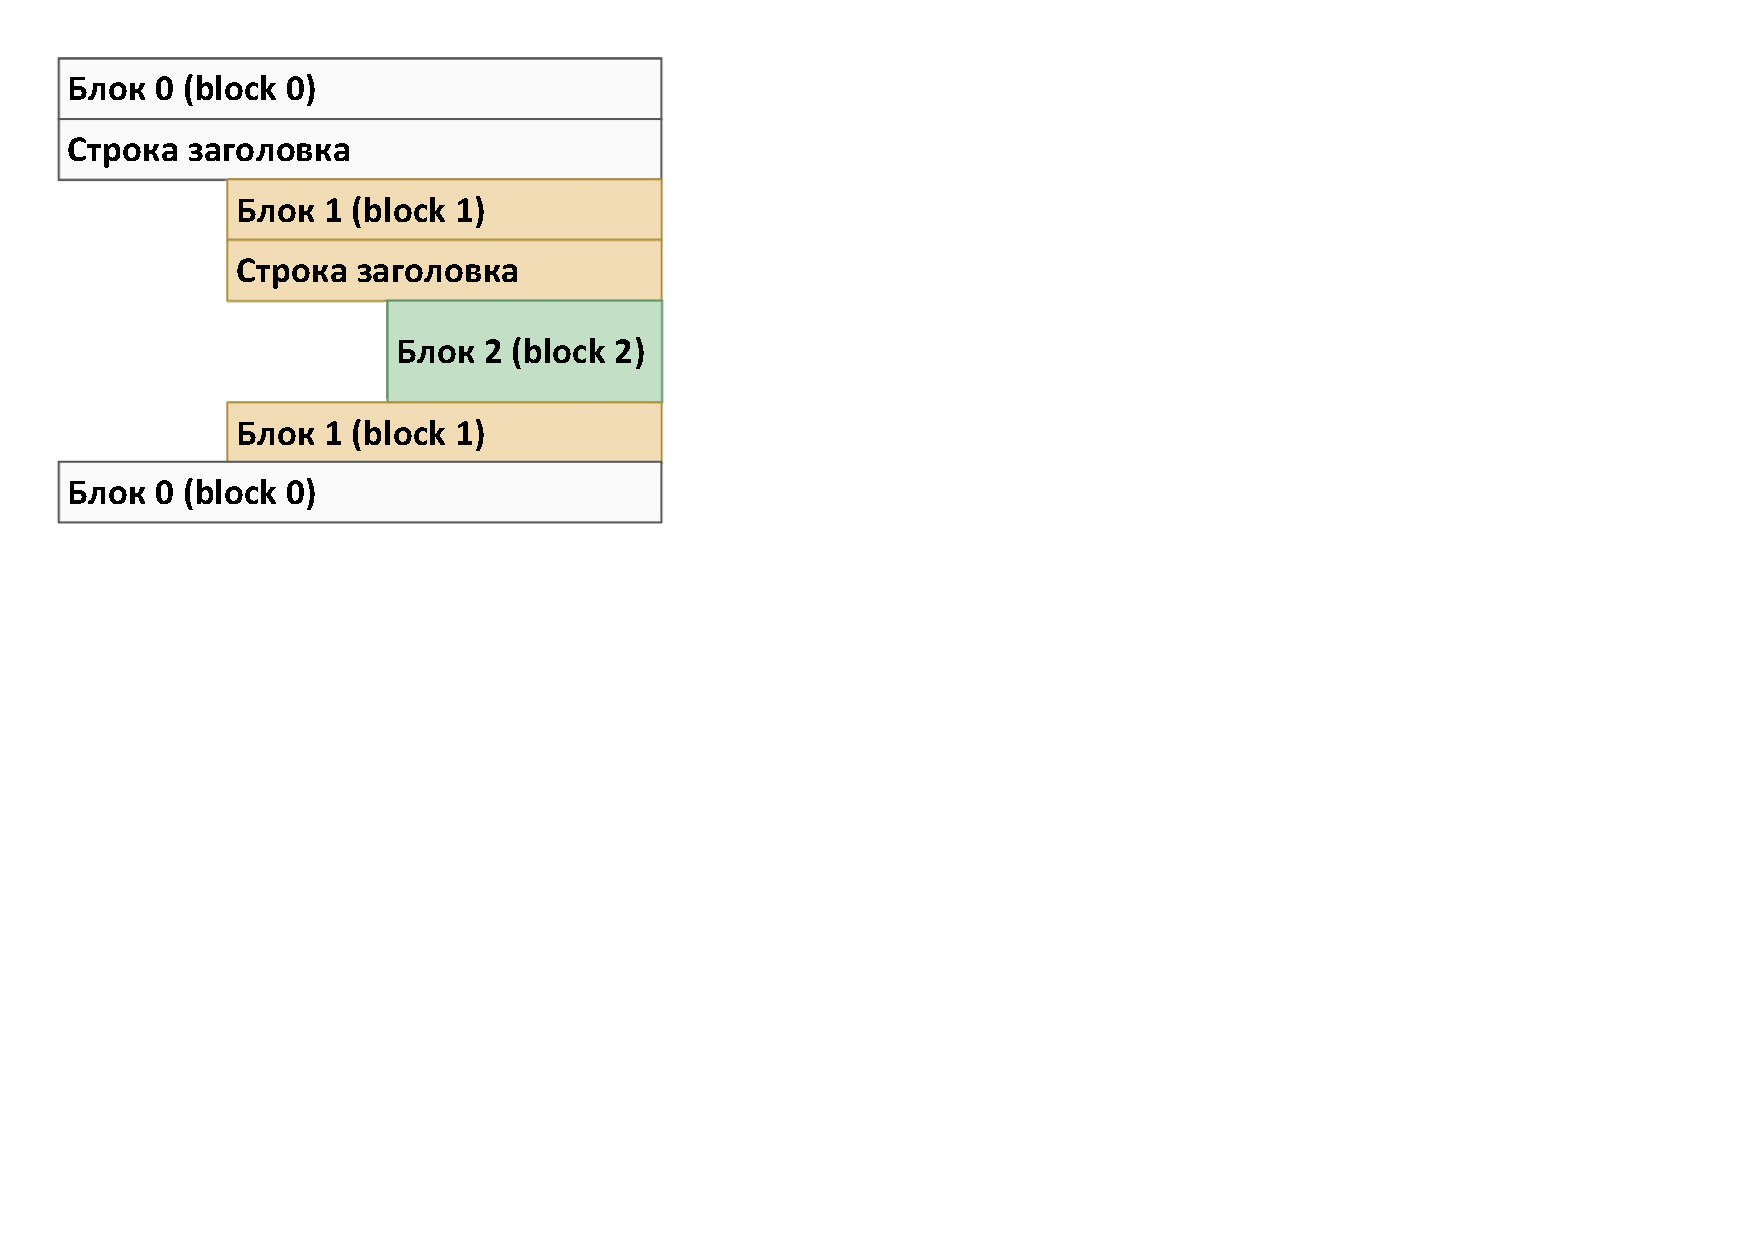
\includegraphics[width=.38\textwidth]{pics/вложенные_блоки_кода}
%
%\end{multicols}	 
%\vfill
%\end{frame}


\section{Тернарное выражение \texttt{if/else}}
\sectionframe


\begin{frame}[fragile]{Тернарное выражение \texttt{if/else}}
\scriptsize
\begin{itemize}
	\item Зачастую элементы, использованные в операторе \mintinline{python}|if|, достаточно просты, так что распространение такого оператора на четыре строки выглядит излишеством.
	
	\item В других случаях конструкцию подобного рода может понадобиться вложить в более крупный оператор, а не присваивать ее результат какой-то переменной.
	
	\item По указанным причинам в Python был добавлен новый формат условного выражения, который позволяет определить то же самое в одном действии (тернарный оператор).
\end{itemize}

\begin{multicols}{2}

\begin{minted}[linenos=true]{python}
if x:
    a = y
else:
    a = z
\end{minted}

\columnbreak

\begin{minted}{python}
a = y if x else z
\end{minted}
\end{multicols}
\vfill
\end{frame}


\begin{frame}[fragile]{Тернарное выражение \texttt{if/else}}
\scriptsize
\begin{minted}{pycon}
>>> x = 'f' if 10 else 't'  # Числа, не равные нулю, истина

>>> print(x)
f

>>> x = 'f' if 0 else 't'  # Ноль - это ложь

>>> print(x)
t
\end{minted}
Использовать тернанрый оператор нужно крайне умеренно и только в тех случаях, когда все его составные части относительно просты, иначе предпочтительнее использовать форму полного оператора \mintinline{python}|if| для облегчения его  будущего модифицирования.
\vfill
\end{frame}


\section{Операторы цикла в Python}
\sectionframe


\begin{frame}[fragile]{Операторы цикла}
\scriptsize	
\begin{itemize}
	\item Алгоритмы решения многих задач требуют некоторого количества повторений своих отдельных частей.
	\item Такие повторяющиеся участки называют циклическими, а операторы языка Python, реализующие соответствующие повторения~-- \textcolor{extraorange}{\textbf{операторами цикла}}.
	\item Цикл состоит из \textcolor{extraorange}{\textbf{заголовка цикла}} и \textcolor{extraorange}{\textbf{тела цикла}}.
	\item Заголовок определяет условие прекращения (или выполнения) цикла, а тело цикла содержит операторы, которые нужно повторять.
\end{itemize}

\bigskip	
Операторы цикла в Python:
\begin{enumerate}
	\item Цикл \mintinline{python}|while|
	\item Цикл \mintinline{python}|for|
\end{enumerate}
\vfill
\end{frame}

\subsection{Цикл \texttt{while}}

\begin{frame}[fragile]{Оператор цикла \texttt{while}}

\scriptsize
\begin{multicols}{2}
\begin{itemize}
	\item Оператор \mintinline{python}|while| многократно повторяет блок операторов до тех пор, пока проверка в заголовочной части оценивается как истина.
	
	\item Управление продолжает возвращаться к началу оператора, пока проверка не даст ложное значение. Когда результат проверки становится ложным, управление переходит на оператор, следующий после блока \mintinline{python}|while|.
	
	\item Если проверка оценивается в ложное значение с самого начала, тогда тело цикла никогда не выполнится и оператор \mintinline{python}|while| пропускается.
\end{itemize}
\columnbreak
\centering
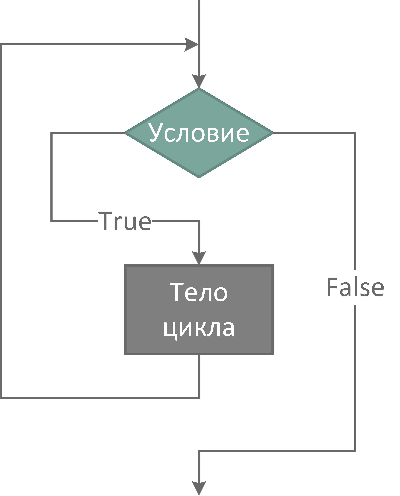
\includegraphics[width=.8\linewidth]{pics/while}
\end{multicols}
\vfill
\end{frame}

\begin{frame}[fragile]{Оператор цикла \texttt{while}}
\scriptsize
Общий формат цикла \mintinline{python}|while|: 

\begin{minted}{python}
while expression:  # Проверка цикла
    operator_1      # Тело цикла
    operator_2
    ...
    operator_n
\end{minted}
Цикл \mintinline{python}|while| можно использовать:
\begin{itemize}
	\item  в математических итерационных алгоритмах для проведения вычислений с заданной точностью;
	\item  при вводе данных, когда их количество заранее неизвестно, а условие завершения ввода определено некоторым введенным значением;
	\item при поиске нужного элемента в какой-либо структуре данных.
\end{itemize}
\vfill
\end{frame}


\begin{frame}[fragile]{Примеры использования цикла \texttt{while}}
\scriptsize
Необходимо написать программу для вычисления $n!$:
\begin{equation*}
	n! = 1 \cdot 2 \cdot 3 \cdot \ldots \cdot \left(n - 1\right) \cdot n
\end{equation*}
где $n$~-- положительное целое число.
\begin{minted}[linenos=true]{python}
n = int(input('Введите положительное целое число: '))

i = 1
f = 1

while i <= n:
    f *= i
    i += 1

print('n! =', f)
\end{minted}
\vfill
\end{frame}


\begin{frame}[fragile]{Примеры использования цикла \texttt{while}}
\scriptsize
Пусть требуется найти максимальное значение среди заранее неизвестного количества вводимых натуральных чисел. При появлении нуля или отрицательного числа ввод завершается. Для диапазона вводимых данных достаточно использовать тип \mintinline{python}|int|.
\begin{minted}{pycon}
>>> max_number, n = 0, 1

>>> while n > 0:
...     n = int(input('Введите натуральное число: '))
...     if n > max_number:
...         max_number = n
...
>>> print('Максимальное число = ', max_number)
Введите натуральное число: 10
Введите натуральное число: 2
Введите натуральное число: 35
Введите натуральное число: 5
Введите натуральное число: 0
Максимальное число =  35
\end{minted}
\vfill
\end{frame}


\subsection{Цикл \texttt{for}}
\scriptsize
\begin{frame}[fragile]{Оператор цикла \texttt{for}}
	\begin{itemize}
		\item Оператор \mintinline{python}|for...in| также является оператором цикла, который осуществляет итерацию по \textcolor{extraorange}{\textbf{последовательности}} объектов, т.е. проходит через каждый элемент в последовательности.
		
		\item \textcolor{extraorange}{\textbf{Последовательность}}~-- это упорядоченный или неупорядоченный набор элементов.
		
		\item Во многих случаях в заголовке цикла \mintinline{python}|for| используется функция \mintinline{python}|range()|, которая является генератором арифметических прогрессий:
	\end{itemize}

\begin{minted}{pycon}
>>> for i in range(10):  # 10 не включительно
...     print(i, end=' ')
0 1 2 3 4 5 6 7 8 9

>>> for i in range(1, 11): # можно задать начальное значение
...     print(i, end=' ')
1 2 3 4 5 6 7 8 9 10

>>> for i in range(0, 11, 2):  # также можно менять шаг
...     print(i, end=' ')
0 2 4 6 8 10
\end{minted}
\vfill
\end{frame}


%\begin{frame}[fragile]{Оператор цикла \texttt{for}}
%\scriptsize
%Функция \mintinline{python}|range()|~-- генератор арифметических прогрессий:
%
%\begin{minted}{pycon}
%>>> for i in range(1, 11): # можно задать начальное значение
%...     print(i, end=' ')
%1 2 3 4 5 6 7 8 9 10
%
%>>> for i in range(0, 11, 2):  # также можно менять шаг
%...     print(i, end=' ')
%0 2 4 6 8 10
%\end{minted}
%\vfill
%\end{frame}


%\begin{frame}[fragile]{Вложенные циклы \texttt{for}}
%\scriptsize
%Операторы цикла \mintinline{python}|for| могут быть вложены друг в друга на произвольную глубину:
%
%\begin{minted}{python}
%|In [1]:| for i in range(3):
%   |...:|     for j in range(3):
%   |...:|         if i != j:
%   |...:|             print(i, j, round(1 / (i + j), 2))
%0 1 1.0
%0 2 0.5
%1 0 1.0
%1 2 0.33
%2 0 0.5
%2 1 0.33
%\end{minted}
%\vfill
%\end{frame}


\section{Операторы \texttt{break}, \texttt{continue}, \texttt{pass} и \\ конструкция \texttt{else} цикла}
\sectionframe


\begin{frame}[fragile]{Оператор \texttt{break}}
\scriptsize
Оператор \mintinline{python}|break| выполняет немедленный выход из цикла, т.е. остановку выполнения команд, даже если условие выполнения цикла еще не приняло значение \mintinline{python}|False| или последовательность элементов не закончилась.

\begin{minted}{pycon}
>>> while True:
...     name = input('Enter name: ')
...     if name == 'stop':
...         break
...     age = input('Enter age: ')
...     print('Hello', name, '=>', int(age) * 2)
Enter name: John
Enter age: 35
Hello John => 70
Enter name: Julya
Enter age: 24
Hello Julya => 48
Enter name: stop
\end{minted}
\vfill	
\end{frame}


\begin{frame}[fragile]{Оператор \texttt{continue}}
\scriptsize	
Оператор \mintinline{python}|continue| используется для немедленного перехода в начало цикла.

\begin{multicols}{2}

\begin{minted}{pycon}
>>> x = 10

>>> while x:
...     x -= 1
...     # Нечетное? Тогда пропустить
...     if x % 2 != 0: 
...         continue  
...     print(x, end=' ')
8 6 4 2 0
\end{minted}

\columnbreak

\begin{minted}{pycon}
>>> x = 10

>>> while x:
...     x -= 1
...     # Четное? Тогда выводим
...     if x % 2 == 0:   
...         print(x, end=' ')
8 6 4 2 0
\end{minted}

\end{multicols}
\vfill
\end{frame}


%\begin{frame}[fragile]{Оператор \texttt{pass}}
%\scriptsize
%\begin{itemize}
%	\item Оператор \mintinline{python}|pass|~-- это заполнитель, обозначающий отсутствие действий, используемый в ситуациях, когда синтаксис требует оператора, но нет возможности выполнить что-либо полезное.
%		
%	\item Данный оператор часто применяется для кодирования пустого тела для составного оператора.
%\end{itemize}
%
%К примеру, с помощью \mintinline{python}|pass| можно написать бесконечный цикл, который на каждом проходе ничего не делает:
%
%\begin{minted}{python}
%while True:
%    pass  # Для прекращения работы нажмите <Ctrl+C>!
%\end{minted}
%\vfill
%\end{frame}


\begin{frame}[fragile]{Конструкция \texttt{else} цикла}
\scriptsize
Полная форма записи циклов \mintinline{python}|while| и \mintinline{python}|for| выглядит следующим образом:

\begin{multicols}{2}

\begin{minted}[linenos=true]{python}
while condition():
    operators

    # Выход с пропуском else
    if exit_test():
        break 

    # Переход к заголовку цикла
    if skip_test():
        continue

# Выполняется, если не было break
else:
    operators
\end{minted}

\columnbreak

\begin{minted}[linenos=true]{python}
for x in collection:
    operators

    # Выход с пропуском else
    if exit_test():
        break 

    # Переход к заголовку цикла
    if skip_test():
        continue

# Выполняется, если не было break
else:
    operators
\end{minted}

\end{multicols}	

Если циклы \mintinline{python}|while| или \mintinline{python}|for| прервать оператором \mintinline{python}|break|, соответствующие им блоки \mintinline{python}|else| выполняться не будут.
\vfill
\end{frame}


%\begin{frame}[fragile]{Конструкция \texttt{else} цикла}
%\scriptsize
%В приведенном примере выполняется проверка, является ли положительное целое число $y$ простым, за счет поиска сомножителей больше 1:
%
%\begin{minted}[linenos=true]{python}
%x = y // 2  # Для y > 1
%
%while x > 1: 
%    if y % x == 0:  # Остаток от деления
%        print(y, "has factor", x)   # Имеет сомножитель
%        break  # Пропуск else
%    
%    x -= 1
%
%else:  # Нормальный выход
%    print(y, "is prime")  # Является простым  
%\end{minted}
%\vfill
%\end{frame}


\section{Примеры}
\sectionframe

\begin{frame}[fragile]{Пример~1}
\scriptsize
Необходимо составить таблицу функции $P(x)$:
\begin{Large}
\begin{equation*}
	P = \tan \left(x \right) + \dfrac{y^2}{\sqrt{k}} - 16.3
\end{equation*} 
\end{Large}
где $k = \sin \left(3 \cdot x\right) + \cos\left(x \right)$; \quad $x = 12.4$.
Значение переменной y изменяется от 2.5 до 4.7 с шагом 0.2. 

\bigskip
Определить количество повторений цикла можно следующим образом:
\begin{equation*}
	n = int \left(\left(stop - start\right)/h\right) + 1
\end{equation*}
где \mintinline{python}|int|~-- стандартная функция Python, которая возвращает целую часть числа, отбросив его дробную часть; \texttt{stop}~-- конечное значение переменной, по которой организуется цикл; \texttt{start}~-- начальное значение переменной, по которой организуется цикл; \texttt{h}~-- шаг изменения переменной, по которой организуется цикл.
\vfill
\end{frame}


\begin{frame}[fragile]{Пример~1}
\scriptsize
\textbf{Решение с помощью цикла} \mintinline{python}|while|
\begin{minted}[fontsize=\fontsize{7pt}{8pt}]{pycon}
>>> import math
>>> start, stop, h = 2.5, 4.7, 0.2
>>> x = 12.4
>>> k = math.sin(3 * x) + math.cos(x)
>>> y = start
>>> while y <= stop:  # y не дойдет до конечного значения
...     p = math.tan(x) + y ** 2 / k ** 0.5 - 16.3
...     print(f'y = {y}, p = {p}')
...     y += h
...
y = 2.5, p = -7.6950436192326155
y = 2.7, p = -6.2352365230954625
y = 2.9000000000000004, p = -4.663136573409297
y = 3.1000000000000005, p = -2.9787437701741197
y = 3.3000000000000007, p = -1.1820581133899317
y = 3.500000000000001, p = 0.7269203969432709
y = 3.700000000000001, p = 2.748191760825481
y = 3.9000000000000012, p = 4.881755978256706
y = 4.100000000000001, p = 7.127613049236945
y = 4.300000000000002, p = 9.485762973766192
y = 4.500000000000002, p = 11.956205751844458
\end{minted}
Для вывода всех значений нужно исправить условие в заголовке: \mintinline{ipython}|while y <= stop + 0.5 * h: ...|
\vfill
\end{frame}

\begin{frame}[fragile]{Пример~1}
\scriptsize
\textbf{Решение с помощью цикла} \mintinline{python}|for|
\begin{minted}[fontsize=\fontsize{7pt}{8pt}]{pycon}
>>> import math
>>> start, stop, h = 2.5, 4.7, 0.2
>>> x = 12.4
>>> k = math.sin(3 * x) + math.cos(x)
>>> y = start
>>> n = int((stop - start) / h) + 1
>>> for _ in range(n):
...     p = math.tan(x) + y ** 2 / k ** 0.5 - 16.3
...     print(f'y = {y}, p = {p}')
...     y += h
...
y = 2.5, p = -7.6950436192326155
y = 2.7, p = -6.2352365230954625
y = 2.9000000000000004, p = -4.663136573409297
y = 3.1000000000000005, p = -2.9787437701741197
y = 3.3000000000000007, p = -1.1820581133899317
y = 3.500000000000001, p = 0.7269203969432709
y = 3.700000000000001, p = 2.748191760825481
y = 3.9000000000000012, p = 4.881755978256706
y = 4.100000000000001, p = 7.127613049236945
y = 4.300000000000002, p = 9.485762973766192
y = 4.500000000000002, p = 11.956205751844458
y = 4.700000000000002, p = 14.538941383471727
\end{minted}
\vfill
\end{frame}


\section{Задания}
\sectionframe


\begin{frame}[fragile]{Задание~1}
\large
Необходимо вычислить f:
\begin{equation*}
\mathrm{
f = \left\{
\begin{aligned}
	& x + \dfrac{x}{x - \dfrac{y}{25 - k}} \cdot \dfrac{\tan \left(k\right)}{\left(k + x\right)^2} + \dfrac{y^2}{\sqrt{k}} &\quad \text{при } -5 \leqslant x < 0; \quad 0 < x \leqslant 3 \\
	& \dfrac{x^3}{y} + a \cdot x ^ {2 - y \cdot x} - \cos^2\left(x\right) + \dfrac{\sqrt[3]{x \cdot y}}{34 - a} &\quad \text{при } x = 0 \\
	& \dfrac{1}{x} \cdot \ln \left(1 + 2 \cdot y\right) + \dfrac{c}{4 - \sqrt[6]{3 \cdot y + 5 \cdot x}} &\quad \text{при } 3 < x \leqslant 5 \\
	& 0 &\quad \text{при } x > 5
\end{aligned}	
\right.}
\end{equation*}

где \quad $\mathrm{a = 26; \quad c = 28.96; \quad y = 1.3; \quad k = 9.86; \quad x \in \left[-5; 6\right]; \quad h = 1}$.
\vfill
\end{frame}


\begin{frame}[fragile]{Задание~2}
\large
Вычислите константу скорости химической реакции k в интервале температур $\mathrm{T \in \left[700; 750\right]}$ (шаг изменения $\mathrm{h = 5 K}$):
\begin{equation*}
	\mathrm{k = k_0 \cdot e^{-E_a / RT}}
\end{equation*}
\begin{equation*}
\mathrm{
	E_a = \left\{
	\begin{aligned}
		& 60, T \leqslant 720 \\
		& 59, 720 < T \leqslant 730 \\
		& 57, 730 < T \leqslant 750
	\end{aligned}
	\right.}
\end{equation*}
$\mathrm{k_0 = 100; \qquad R = 8.314}$.
\vfill
\end{frame}


\begin{frame}[fragile]{Задание~3}
\large
Вычислите давление насыщенных паров углеводородов $C_{6_{+}}$ (P) в сепараторе по формуле Аш-Ворта:
\begin{equation*}
	\mathrm{P = \exp \left(2.3 \cdot \left(2.68 \cdot \left(1 - \dfrac{f_2}{f_1}\right)-1\right)\right)}
\end{equation*}
\begin{equation*}
\mathrm{
	f_1 = \left\{
	\begin{aligned}
		& \mathrm{\sqrt{\left(68.74 + 273.15\right)^2 + 1.08 \cdot 10^3} - 308.6, T \leqslant 11.4} \\
		& \mathrm{\sqrt{\left(124.7 + 273.15\right)^2 + 1.08 \cdot 10^3} - 308.6, 11.4 < T \leqslant 37.8} \\
		& \mathrm{\sqrt{\left(134.7 + 273.15\right)^2 + 1.08 \cdot 10^3} - 308.6,  37.8 < T}
	\end{aligned}
	\right.}
\end{equation*}
\begin{equation*}
\mathrm{
	f_2 = \dfrac{1250}{\sqrt{\left(T+273.15\right)^2 + 1.08 \cdot 10^3} - 307.6} - 1
}
\end{equation*}
T изменяется в интервале 10-40°С с шагом 2.5°С.
\vfill
\end{frame}


\contactsframe[\Large \textbf{Благодарю за внимание!}]{
	
	
\includegraphics[width=.05\textwidth]{pics/home} \quad Учебный корпус №2, ауд. 136 \\
	
\includegraphics[width=.05\textwidth]{pics/mail} \quad chuva@tpu.ru \\
	
\includegraphics[width=.03\textwidth]{pics/tel} \quad +7-962-782-66-15
}

\end{document}

